\section {Ambiente virtual}

\subsection{ Melhora da Usabilidade e Imersão no ambiente virtual }

Após o término do desenvolvimento do ambiente virtual, viu-se a necessidade de uma melhora na usabilidade e imersão, por parte do usuário, no ambiente virtual. Durante os testes realizados pela equipe foram encontrados alguns problemas como: a grande distância entre os pontos chave do ambiente virtual, onde o usuário deveria de locomover por quilômetros para atravessar todo o mapa desenvolvido; a grande largura das trilhas, que acabavam que não guiavam muito bem o usuário durante o percurso; o fato do usuário poder sair dos limites da trilha proposta e se adentrar em lugares não planejados e projetados para isso; alguns objetos do ambiente eram desproporcionais entre si, sendo alguns objetos muito grandes e outros muito pequenos; as informações apresentadas para o usuário, como velocidade, não estavam em um local adequado.

Tendo em vista as dificuldades anteriormente encontradas para a utilização do ambiente virtual, foram feitas algumas melhorias a fim de maximizar a boa experiência do usuário no contexto do Bike-X. A seguir, são apresentadas as soluções adotadas:

O ambiente virtual como um todo foi reduzido, para que o usuário consiga realizar todo o percurso em um tempo e uma distância aceitáveis, sem valores absurdos. A figura \ref{fig:mapaReduzido}, mostra a visão superior do mapa desenvolvido para o ambiente virtual.

\begin{figure}[h]
  \centering
  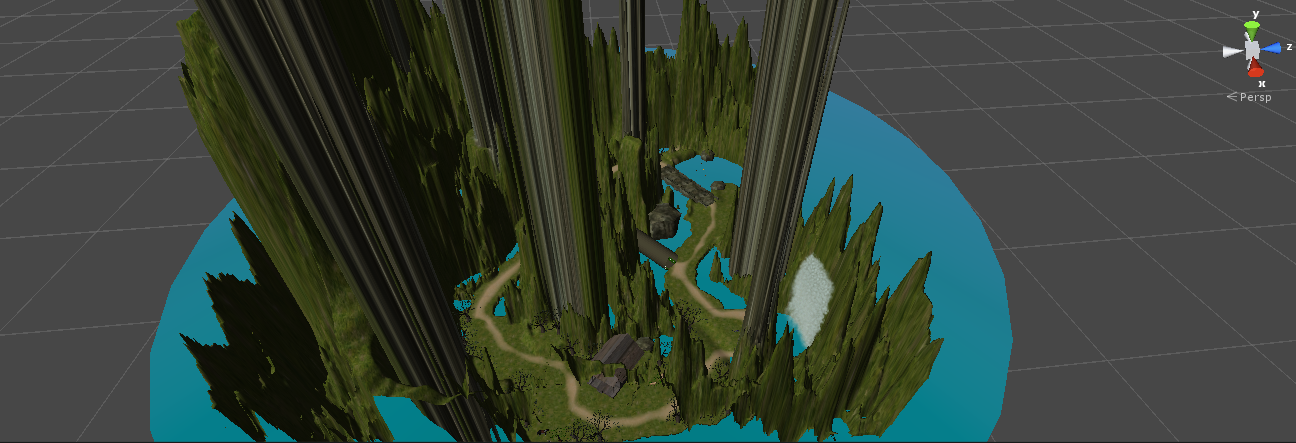
\includegraphics[width=0.5\textwidth]{figuras/mapaReduzido}
  \caption{Visão superior do mapa reduzido}
  \label{fig:mapaReduzido}
\end{figure}

As trilhas se tornaram mais estreitas, norteando de uma melhor maneira o usuário no decorrer do percurso. Além disso, foram adicionados alguns objetos adjacentes ao percurso a fim de melhorar a experiência do usuário, como os animais ilustrados na figura \ref{fig:animaisPista}. Os animais apresentados apresentavam problemas de proporção com o resto do ambiente virtual, com isso, a escala de tamanho dos mesmos foi reduzida.

\begin{figure}[h]
  \centering
  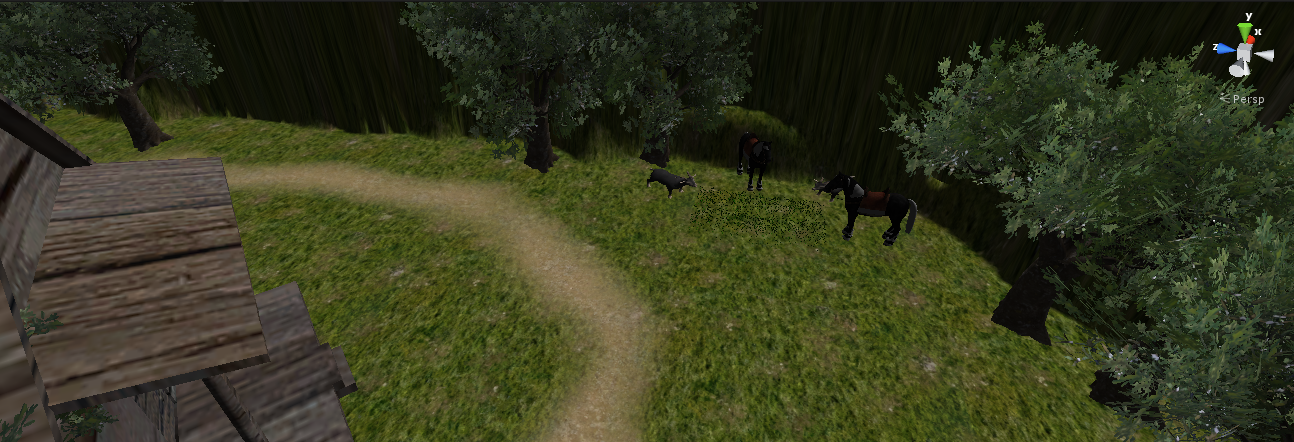
\includegraphics[width=0.5\textwidth]{figuras/animaisPista}
  \caption{Visão da trilha com animais adjacentes}
  \label{fig:animaisPista}
\end{figure}

Como pode ser visto nas figuras \ref{fig:blocosPercurso} e \ref{fig:blocosColisao}, foram criados vários blocos de colisão ao redor de toda a trilha para que o usuários não possa atingir lugares inadequados, como a água. Essa solução foi implementada utilizando planos invisíveis para o usuário, que o impedirá de ultrapassar determinados limites. A utilização de planos foi a forma mais fácil, identificada pela equipe, de se contornar o problema enfrentado.

\begin{figure}[h]
  \centering
  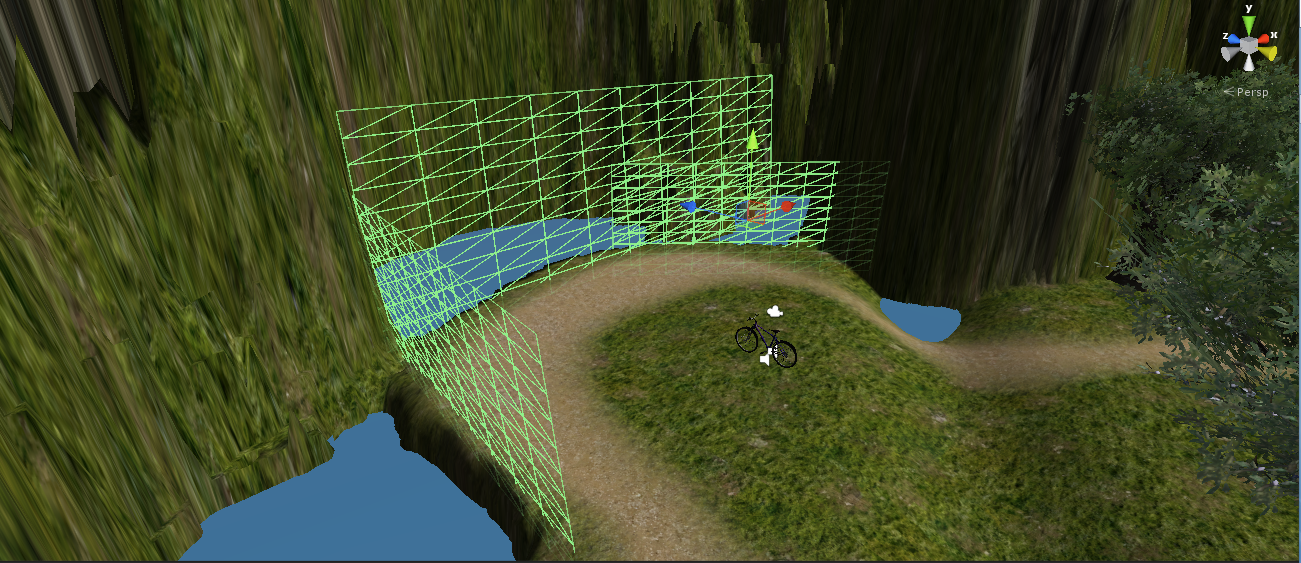
\includegraphics[width=0.5\textwidth]{figuras/blocosColisao}
  \caption{Blocos de Colisão}
  \label{fig:blocosColisao}
\end{figure}

\begin{figure}[h]
  \centering
  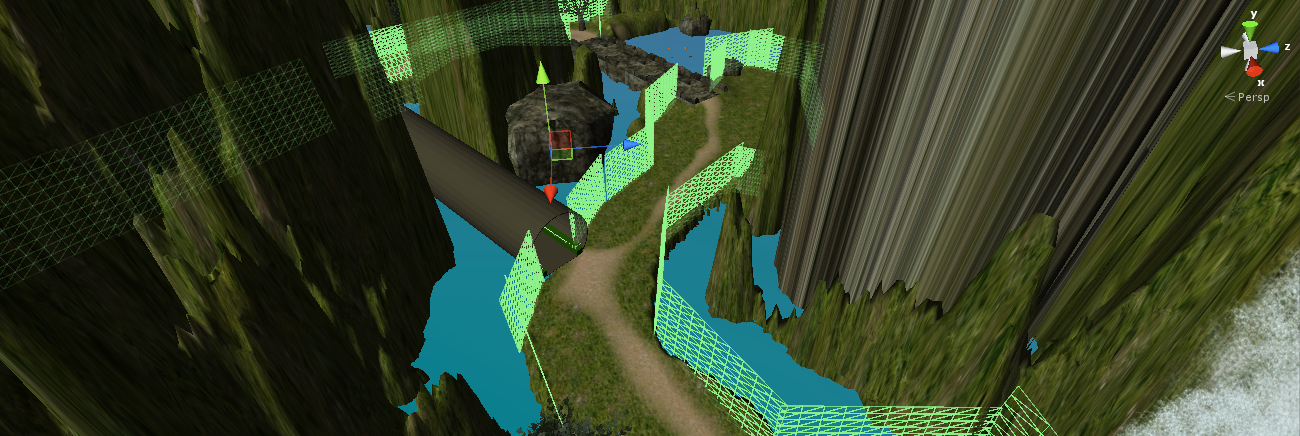
\includegraphics[width=0.5\textwidth]{figuras/blocosPercurso}
  \caption{Blocos de Colisão no decorrer do percurso da trilha}
  \label{fig:blocosPercurso}
\end{figure}

Depois da criação dos blocos de colisão para impedir que o usuário ultrapasse locais indevidos foi acrescentado ao ambiente \textit{ MeshRenderCollider } de colisões de objetos nas pontes, pedras, animais, árvores e na casa, assim quando o usuário tentar colidir com uma casa ou com um animal , ou ao mesmo atravessar a ponte ou o túnel ele não irá passar por dentro do mesmo e sim por cima, permitindo a travessia, como pode ser visto nas figuras \ref{fig:bridgePosition}, \ref{fig:newTunnel
} e \ref{fig:animalsCollider}.

\begin{figure}[h]
  \centering
  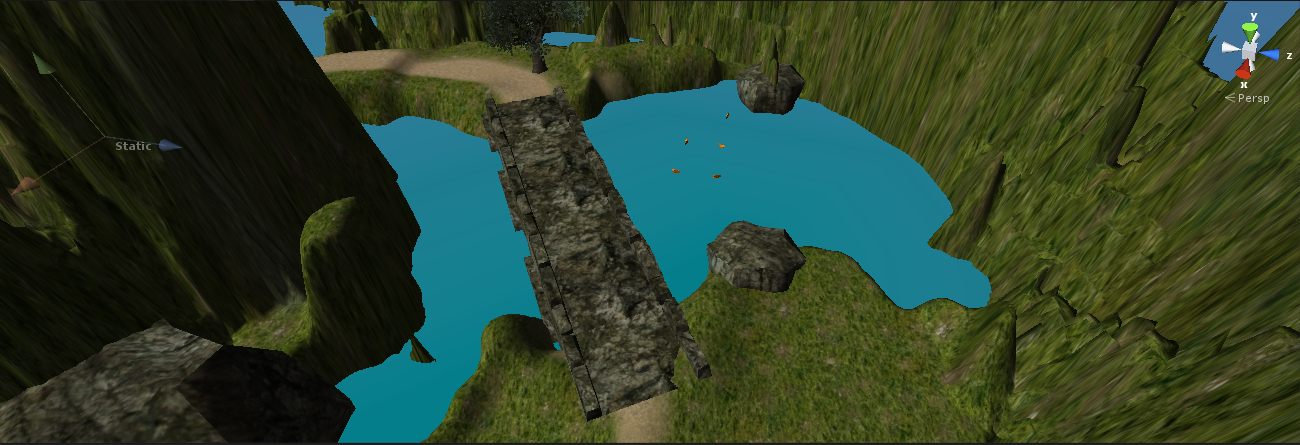
\includegraphics[width=0.5\textwidth]{figuras/bridgePosition}
  \caption{Ponte utilizada no ambiente virtual}
  \label{fig:bridgePosition}
\end{figure}

\begin{figure}[h]
  \centering
  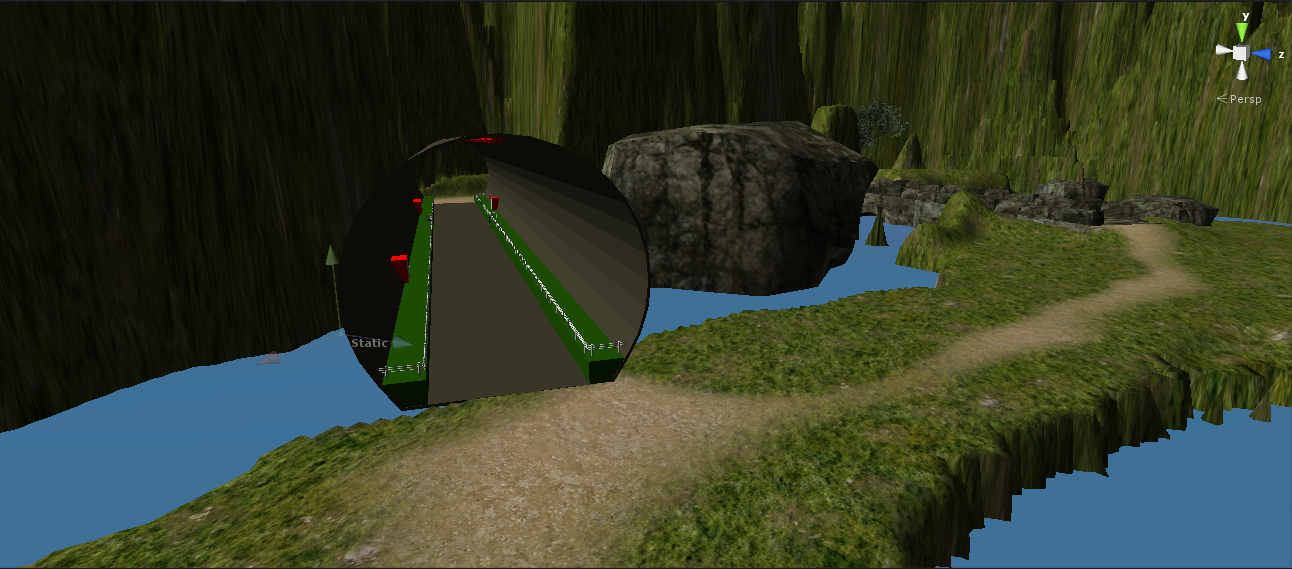
\includegraphics[width=0.5\textwidth]{figuras/newTunnel}
  \caption{Túnel utilizado no ambiente virtual}
  \label{fig:newTunnel}
\end{figure}

\begin{figure}[h]
  \centering
  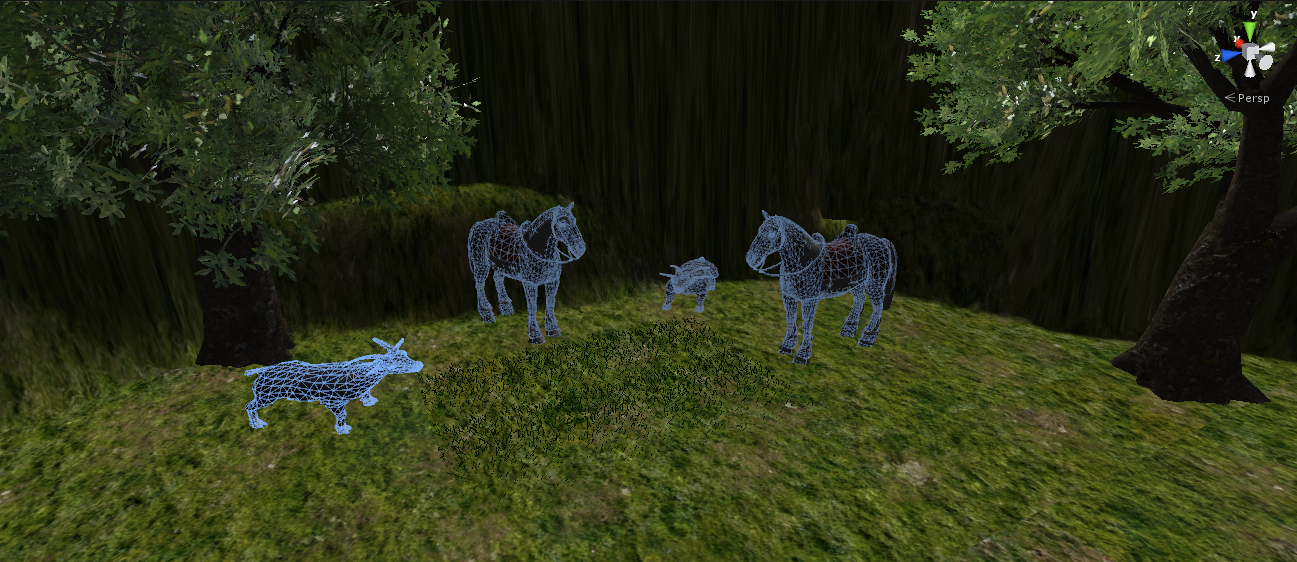
\includegraphics[width=0.5\textwidth]{figuras/animalsCollider}
  \caption{Colisão nos animais adjacentes a trilha}
  \label{fig:animalsCollider}
\end{figure}

Para melhorar ainda mais a experiência do usuário foram adicionados sons de natureza no ambiente virtual, como o som da cachoeira que foi adicionada ao percurso (figura \ref{fig:waterFallPosition}) e de corrente de água ao atravessar a ponte.

\begin{figure}[h]
  \centering
  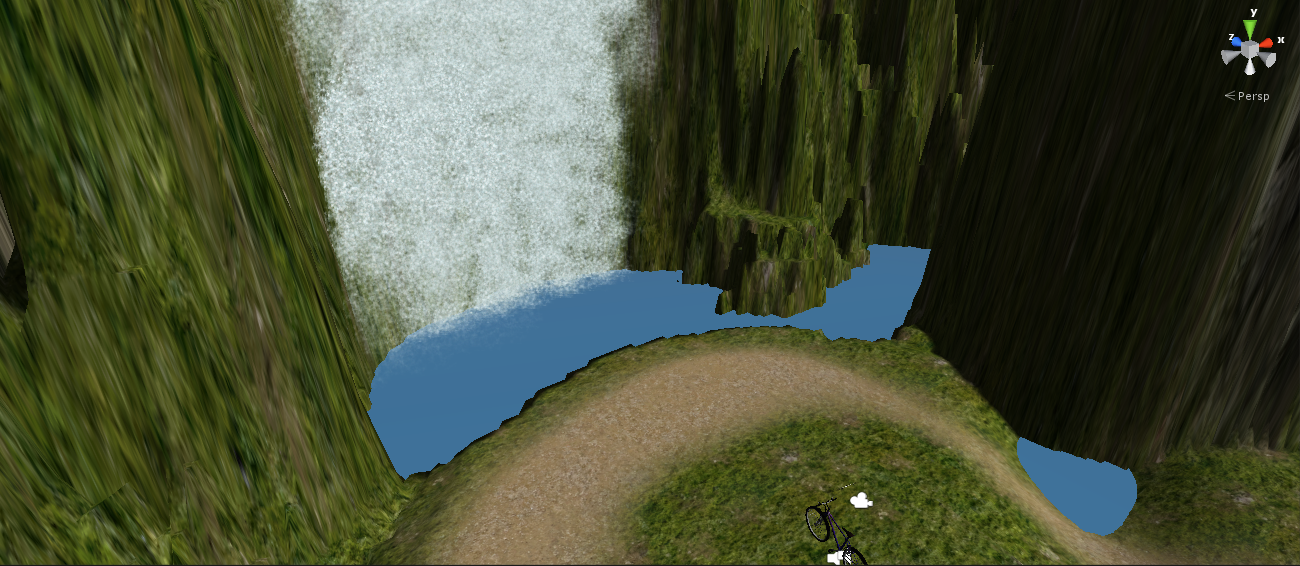
\includegraphics[width=0.5\textwidth]{figuras/waterFallPosition}
  \caption{Cachoeira presente no decorrer da trilha}
  \label{fig:waterFallPosition}
\end{figure}

A principal dificuldade encontrada pela equipe foi em como apresentar as informações para o usuário na tela sem comprometer a interação com o ambiente virtual. Preferiu-se então apresentar de uma maneira bem simples, através de uma caixa de diálogo no canto superior direito da tela, como pode ser visto na figura \ref{fig:improvedInterface}, ao invés de apenas adicionar as informações no centro da tela.


\begin{figure}[h]
  \centering
  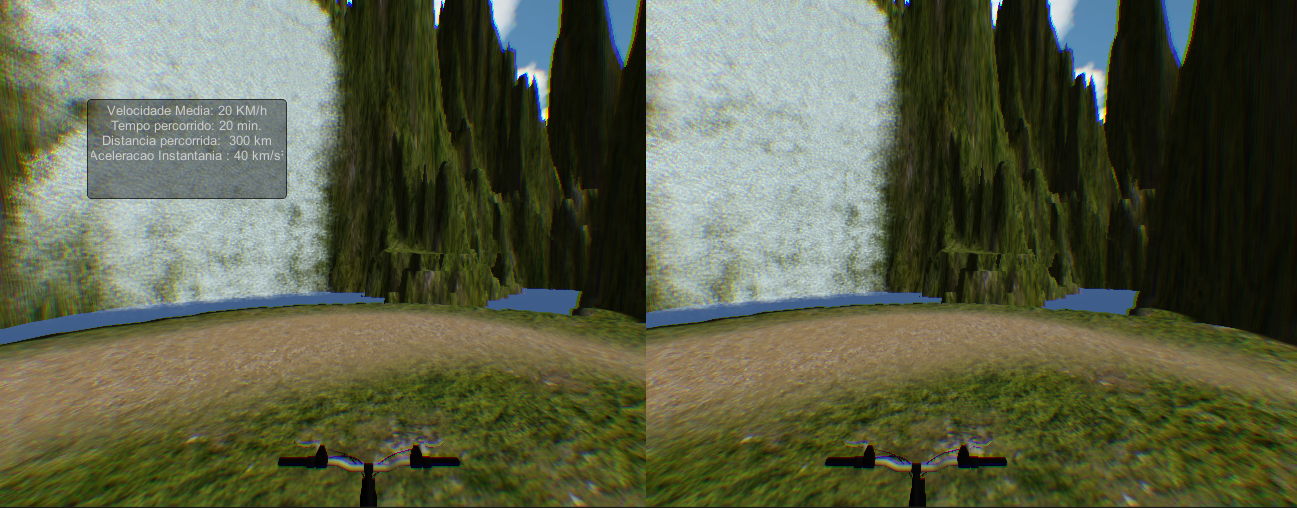
\includegraphics[width=0.5\textwidth]{figuras/improvedInterface}
  \caption{\textit{Interface} com o usuário para apresentação de informações}
  \label{fig:improvedInterface}
\end{figure}

